
\documentclass[openany,oneside,12pt,hidelinks]{book}
\usepackage[unicode]{hyperref}
\usepackage[utf8]{inputenc}
\usepackage{geometry}
\usepackage{amsmath, amssymb}
\usepackage{graphicx}
	\graphicspath{{./Images}}
\usepackage{marginnote}
\usepackage{parskip}
\usepackage{tikz} 
\usetikzlibrary{calc,arrows.meta,decorations.pathreplacing}
\usepackage{setspace}
\usepackage{csquotes}
\usepackage{caption}
\usepackage{dirtytalk} 
\usepackage[
backend=biber,
style=alphabetic,
sorting=ynt]{biblatex}
\addbibresource{references.bib} 
%Document Organisation: 
\author{Zain Sikand}
\title{Problem Catalogue}
\geometry{a4paper,portrait, margin=2cm}
\date{2025-2027}
%Starting Document:  
\begin{document}
\begin{raggedright}
  %Formatting: 
  \pagenumbering{arabic}
  \maketitle
  \tableofcontents
  \newpage
  %Introduction: 
  \section{Introduction:}
  A collection of hellish maths and physics problems, lacking boundarie and pushing the will of an A-Level student. These problems break down their understanding of maths and physics fundamentally. No form of revision or study at their age aids in the misery bestowed upon them via these problems.
  %Section 1: 
  \chapter{Mathematics}
  \textit{\emph{Definition:} Mathematics,} \textbf{The foundational means to which we, as a lost species amongst the cosmos, attempt to rationalise our existence, attempt to control reality, and attempt to legitimise our purpose as a species.}

  \newpage
  \section{Integrals}
  \subsection{\underline{Problem One:}} \par

  \textbf{\emph{Problem Author: Zain Sikand}} \\
  \textit{Your final answer should be a single expression in the form \(I_1=[h(x)]_{a}^{b}\) where b and a are bounds of \(I_1\) to be found}
  \newline \\
  Conclude whether or not the below integral, \(I_1:\)
  \[I_{1}= \int_{\int_{x}^{2x}(\ln x)^{2}}^{(3+x)^{6}}(\frac{1}{3e^{x}\cos x \sec^{2} x} + \cot x \csc x) \ dx \]
  can be written as a single expression, with all integration expressions evaluated.
  \newline \\
  {Your conclusion must be supported, \textbf{either}, by an attempt to evaluate the integral or, a proof that  \(I_{1}\) has no real anti-derivative.}
  \newline \\
  \textit{[6 Marks]} \\
  \newpage
  \subsubsection{Worked Solution:}
  \[I_{1} = \int_{\int_{x}^{2x}(lnx)^{2}}^{(3+x)^{6}}(\frac{1}{3e^{x}\cos x \sec^{2} x} + \cot x \csc x) \ dx \]
  \(\Rightarrow \ I_{1}=\int_{b}^{a} f(x) dx\) \\

  \(\therefore \ let \ I_{2}=b\) \\
  \[I_2=\int_{x}^{2x}(\ln|x|)^{2}= \int^{2e^{u}}_{e^{u}}u^{2}e^{u}du=[u^{2}e^{u}]^{2e^{u}}_{e^{u}}-\int^{2e^{u}}_{e^{u}}2ue^{u}e^{u}du\] \\
  \[= [u^{2}e^{u}]^{2e^{u}}_{e^{u}}- ([2ue^{u}]^{2e^{u}}_{e^{u}}- \int ^{2e^{u}}_{e^{u}}2e^{u}du=[u^{2}e^{u}] ^{2e^{u}}_{e^{u}}-[2ue^{u}-2e^{u}]^{2e^{u}}_{e^{u}}=[u^{2}e^{u}-2ue^{u}-2e^{u}]^{2e^{u}}_{e^{u}}\] \\
  \[=[x(\ln |x|)^{2}-2x\ln|x|-2x]^{2x}_{x} \because u=\ln|x| \Rightarrow e^{u}=x \] \\
  \(\therefore I_2=x[2(\ln |2x|)^{2}-(\ln |x|)^{2}-\ln |16x^{2}|]\) (\text{This result \(\rightarrow\) from evaluating the bounds}) \\
  \[I_1= \int^{(3+x)^{6}}_{I_{2}} (\frac{1}{3e^{x}\cos x \sec^{2} x} + \cot x \csc x) \ dx = \int^b_a(\frac{1}{3e^{x}\cos x \sec^{2} x)} + \int^{b}_{a} \cot x \csc x\] \\
  \[let \ I_{3}= \int^b_a(\frac{1}{3e^{x}\cos x \sec^{2} x)} = \int^b_a(\frac{1}{3e^{x}\sec x)}dx = \frac{1}{3} \int^b_a(e^{-x}\cos x)dx\] \\
  \[I_{3}=1/3(J) \] \\
  \[J=[-e^{-x}\cos x]^b_a - \int^b_a -e^{-x}\sin x = [-e^{-x}\cos x]^b_a-([-e^{-x}\sin x]^b_a-\int^b_ae^{-x}cosx\] \\
  \[J=[-e^{-x}\cos x]^b_a-[e^{-x}\sin x]^b_a-J \] \\
  \[\therefore \ J=\frac{1}{2}[e^{-x}\sin x-e^{-x}\cos x]^b_a\] \\
  \[\therefore \ I_{3}=\frac{1}{6}[e^{-x}\sin x-e^{-x}\cos x]^b_a\] \\
  \[I_{1}=I_{3}+\int^b_a\cot x \csc x \ dx\] \\
  \[ let \ I_{4}= \int^b_a\cot x \csc x \ dx\] \\
  \[I_{4}= \int^b_a (\frac{1}{\sin x})(\frac{\cos x}{\sin x}) \ dx = \int^b_a \frac{\cos x}{1-\cos^{2} x} \ dx \] \\
  \textbf{Integrate \(I_4\) by parts:}
  \[ I_{4}=\int^b_a \frac{\cos x}{\sin^{2} x} \ dx\] \\
  \[= \int^b_a \cos x ( \frac{1}{\sin^{2} x}) \ dx = [\frac{1}{\sin x}]^b_a-\int^b_a \sin x ( \frac{-2\sin x\cos x}{\sin^{4} x}) \ dx = [\frac{1}{\sin x}]^b_a-\int^b_a \frac{-2 \cos x}{\sin x} \ dx \] \\
  \[ \therefore I_{4}= [\frac{1}{\sin x}]^b_a+ 2I_{4}\] \\
  \[\Rightarrow I_{4}=-\frac{1}{\sin x} \]
  \[ \therefore I_{1}= [I_{3}+I_{4}]^b_a \]
  \(\therefore\) The integral \(I_{1}\) can be written as a single expression within its bounds
  \(\therefore\) Q.E.D
  \subsection{\underline{Problem Two:}}
  \textbf{\emph{Modified Daily Integral: Evil}}
  \newline \\

  A tank is formed by rotating the line segment joining \((y,\rho)=(0,1)\) and \((6,2)\)
  in the \((y,\rho)\) plane (height \(y\), radius \(\rho\)) about the \(y\)–axis.
  The tank has height \(6\,\mathrm{m}\) and is completely full at time \(t=0\).
  There is no inflow, and water drains through a valve at the bottom.

  Let \(h\) denote the depth of water measured upward from the bottom
  (\(0 \le h \le 6\)), and let \(r\) be the radius of the water surface when the depth is \(h\).
  Let \(V(h,r)\) denote the volume of water at that moment.

  Conservation of volume gives
  \[
    \frac{dV}{dt}=-Q_{\mathrm{out}}(h),
  \]
  where \(Q_{\mathrm{out}}(h)\) is the volumetric outflow rate in \(\mathrm{m}^3/\mathrm{min}\).

  The valve operates in two phases.
  In each phase the outflow is constant, and its value is given by a definite integral:

  \medskip

  \textbf{Phase I} (for \(6 \ge h \ge 3\)):
  \[
    Q_{\mathrm{out}}(h)=K_{1}, \qquad
    K_{1}=c_{1}\int_{-\infty}^{\infty}
    \frac{|\ln|x||}{(x^{2}+1)(x-1)}\,dx,
    \qquad
    c_{1}=0.12\ \text{(m}^3/\text{min per unit integral)}.
  \]

  \medskip

  \textbf{Phase II} (for \(3>h\ge 0\)):
  \[
    Q_{\mathrm{out}}(h)=K_{2}, \qquad
    K_{2}=c_{2}\int_{0}^{\pi/2} x^{3}\tan x\,dx,
    \qquad
    c_{2}=0.15\ \text{(m}^3/\text{min per unit integral)}.
  \]

  \medskip

  Determine the sum of the magnitudes of the rates at which the water height
  is decreasing when \(h=4.25\) and when \(h=1\).\\

  \subsection{\underline{Problem Three:}}
  \textbf{\emph{Problem Author: Carl Johan Malmsten- 1842}}
  \newline \\
  Evaluate the following integral \(I\), using a related integral if necessary
  \[\int^{\infty}_{1} \frac{\ln(\ln|x|)}{1+2x\cos(\alpha)+x^{2}}dx; \  where \ -\pi\leq \alpha \leq \pi \]

  Information regarding solving the integral, methods used in doing so, and the solution itself
  can be found in \cite{abdulsalam2022new}
  \\
  \newpage
  \section{Euclidian Geometry}
  \subsection{\underline{Problem One:}}
  \textbf{IMO 2011}

  Let \(S\) be a finite set of at least two points in the plane. Assume that no three points of \(S\) are collinear. A windmill is a process that starts with a line \(\ell\) going through a single point \(P \in S\). The line rotates clockwise aboutthe pivot \(P\) until the first time that the line meets some other point belonging to S. This point, \(Q\), takes over as the new pivot, and the line now rotates clockwise about \(Q\), until it next meets a point of \(S\). This process continues indefinitely. Show that we can choose a point \(P\) in \(S\) and a line \(\ell\) going through \(P\) such that the resulting windmill uses each point of \(S\) as a pivot infinitely many times.

  \textit{[12 Marks]} \\

  \subsection {\underline{Problem Two:}}
  \textbf{\emph{Problem Author: Zain Sikand}}
  \newline \\

  Imagine Let \(T_{1}\) be a tetrahedron and let \(S_{1}\) be its circumsphere with radius \(R\).
  For each radius of \(S_{1}\), extend it to a full line and denote this line by \(\ell\).

  In the plane \(z = 0\), consider a circle \(C_{1}\) which circumscribes an equilateral triangle whose sides are tangent to the coordinate axes \(x = 0\) and \(y = 0\).  Thus the triangle has one vertex at the origin and its other two vertices lie on the positive coordinate axes.

  Suppose that for certain choices of the radius of \(S_{1}\), the corresponding line \(\ell\) intersects the plane \(z = 0\) and is tangent to the circle \(C_{1}\).  The set of all such tangent lines \(\ell\) is finite.

  Determine, in terms of \(R\), the area of the circle \(C_{1}\).

  \subsection{\underline{Problem Three:}}
  \textbf{\emph{Problem Author: Carter Owen}}
  \newline \\
  Figure 1.1 shows a right-angled triangle \(\triangle ABC\) of height \(H\), divided vertically by a straight line \(\ell\) such that it meets the triangle at a point defined by the variable \(\phi\). The division of \(\triangle ABC\) splits it at \(\phi\) into a trapezium \(CD{\phi}A\) and a new right angled triangle \(\triangle DB{\phi}\). Deduce the value(s) for \(\phi\) that divides \(\triangle ABC\) such that the area of \(CD{\phi}A\) is equal to that of \(DB{\phi}\).
  \begin{center}
    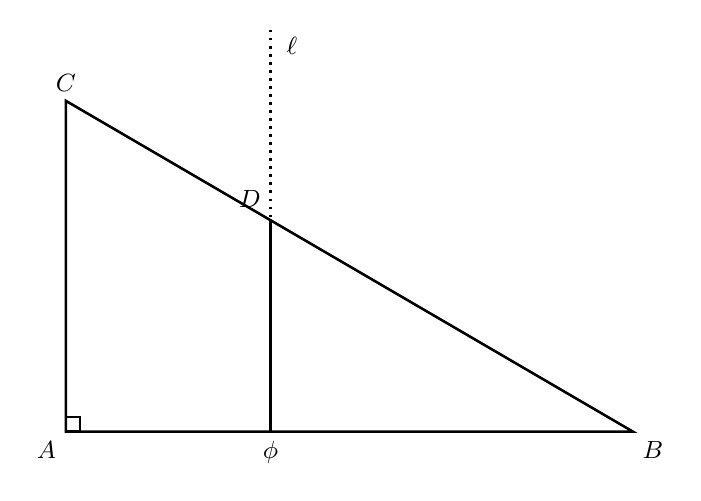
\begin{tikzpicture}[scale=1, font=\small]

      % Internal geometry (not printed)
      \def\b{7.2}        % base length (internal)
      \def\H{4.2}        % height (internal)
      \def\phival{2.6}   % internal numeric x-position of dividing line

      % Main triangle vertices
      \coordinate (A) at (0,0);
      \coordinate (B) at (\b,0);
      \coordinate (C) at (0,\H);

      % Intersection of the vertical line with the hypotenuse = D
      \coordinate (D) at (\phival, {\H*(1 - \phival/\b)});
      % Intersection with the base (labelled phi)
      \coordinate (P) at (\phival,0);

      % a little extra height for the dotted extension above the triangle
      \coordinate (Top) at (\phival, {\H + 0.9 });

      % Draw the triangle outlines
      \draw[line width=0.9pt] (A) -- (B) -- (C) -- cycle;

      % small right-angle box at A
      \draw[line width=0.8pt] (0.18,0) -- ++(0,0.18) -- ++(-0.18,0) -- ++(0,-0.18) -- cycle;
      % Solid segment INSIDE the triangle: from D down to base point P
      \draw[line width=0.9pt] (D) -- (P);

      % Dotted extension ABOVE the triangle: from Top down to D (dotted)
      % label \ell near the dotted part above D
      \draw[dotted, line width=0.9pt] (Top) -- (D) node[pos=0.14, right=2pt, yshift=4pt] {\(\ell\)};

      % re-draw region boundaries to ensure consistent stroke weights
      \draw[line width=0.7pt] (A) -- (P); % left base segment
      \draw[line width=0.7pt] (P) -- (B); % right base segment
      \draw[line width=0.7pt] (A) -- (C); % left vertical
      \draw[line width=0.7pt] (C) -- (D); % left part of hypotenuse
      \draw[line width=0.7pt] (D) -- (B); % right part of hypotenuse

      % Labels: A, B, C
      \node[below left]  at (A) {\(A\)};
      \node[below right] at (B) {\(B\)};
      \node[above] at (C) {\(C\)};

      % Label D at intersection (slightly above-left to avoid overlap)
      \node[above left, yshift=1pt] at (D) {\(D\)};

      % Label the base intersection as phi (symbol only)
      \node[below] at (P) {\(\phi\)};

    \end{tikzpicture}
  \end{center}
  \captionof{figure}{}
  \subsection{\underline{Problem Four:}}
  \textbf{\emph{Moscow State University, 1989}} \\
  In a Trapezium KLMN, sides \(KN\) and \(LM\) are paralell, with \(KN=3\) and \(M= \angle 120^{\circ} \). \(LM\) and \(MN\) are tangent to the circle circumscribed about \(\triangle KLN\). Find the area of \(\triangle KLN\). \\
  \textit{[6 Marks]}
  \newpage
  \section{Real Analysis}
  \subsection{\underline{Problem One:}}
  \textbf{\emph{IMO 2022}}
  \newline \\
  Let \(\mathbb{R^{+}}\) denote the set of positive real numbers. Find all functions \(f : \mathbb{R}^{+} \rightarrow \mathbb{R}^{+}\) such
  that for each \(x \in \mathbb{R^{+}}\), there is exactly one \(y \in \mathbb{R^{+}}\) satisfying \[ xf(y)+yf(x) \leq 2\]

  \chapter{Physics}
  \textit{\emph{Definition:} Physics,} \textbf{The study of all things that exist to place one under  mental, spiritual, and physical duress}
  \newpage
  \section{Kinematics and Further Mechanics}
  \subsection{\underline{Problem One:}}
  \textbf{\emph{Problem Author: Zain Sikand}}
  \newline \\
  A person moving at speed \(S\) whistles, stopping once after 5 seconds of walking. \(t=15s\) later, he continues walking along his current trajectory before passing a stationary group of people. The group of people begin to hear the whistling at \(t=30s\) before he passes them. Determine the speed at which the man is walking, assuming the \textbf{speed of sound= \(330ms^{-1}\)}
  \newpage
  \section{Astrophysics}

  \subsection{\underline{Problem One:}}
  \textbf{\emph{BAAO 2022-23}}
  \newline \\
  The very first image released by the JamesWebb Space Telescope (JWST) was of a galaxy cluster
  called SMACS 0723. The image is considered to be Webb’s first deep field, since a long exposure
  time of 12.5 hours was used to allow the light from very faint and distant galaxies to be seen. The
  spectrum of one such galaxy is shown in Figure 2.1.
  \newline \\

  \begin{center}
    \makebox[\textwidth]{\includegraphics[width=1.0\textwidth]{Figure2-1}}
  \end{center}

  \captionof{figure}{Highly redshifted emission lines in the spectrum of a galaxy that is 13.1 billion years old, captured
    using the JWST’s near-infrared spectrometer (NIRSpec). Credit: NASA, ESA, CSA, STScI.\\}

  The spectrum shows four bright hydrogen lines, which are part of the Balmer series (some of
  which are normally seen in the visible). The rest frame wavelengths of the longest four lines in
  the series are 410 nm, 434 nm, 486 nm and 656 nm \textbf{(not all of which are visible in the spectrum)}. \\
  Once a redshift is known, its recessional velocity can be calculated. At very high redshifts, such
  as these, General Relativity must be used.\\
  A conversion from redshift to recessional velocity is
  shown in Figure 3.
  \newline \\

  a) Taking measurements from the spectrum, estimate the redshift of the galaxy. \emph{[Hint: you
        should measure more than one line to ensure you correctly identify which rest frame
        wavelength corresponds to which line.]}
  \newline \\

  b) Taking the value of the Hubble constant to be \(H_{0} = 70kms^{-1}Mpc^{-1}\), what is the distance
  to the galaxy? Give your answer in Mpc. \\

\chapter{Philosophy}
  \newpage
  \section{Principles Regarding Infinity}
  \subsection{\underline{Human Knowledge}}
  George Berkeley, in his \emph{Treatise Concerning the Principles of Human Knowledge}, explores the idea that man is disillusioned by the incomprehensible nature of infinity, a conciousness that is finite is incapable of comprehending that of the infinite. From this, he goes on to reject the notion of abstract, mind-independent material substance given that it is incomprehensible to a finite being. He, instead, asserts that reality consists only of finite minds and infinite minds- with god's boundless perception being the primary reason for the conceptualisation of the infinite.
  \newline \\
  Shifting to a mathematical perspective, we see Berkeley reject the mathematical interpretations of infinitesimals and infinite quantities, he believes them to be incoherent and undefineable within man's finite perception of reality.
  This is seen in how he attacks the notion of \textbf{fluxions}, referring to them as the \say{ghosts of departed quantities}.
  Further exploring this idea of the comprehensibility of that of the infinite, we can see that his perspective regarding such critiques the usage of abstraction in order to conceptualise.
  He attacks the notion of \say{infinitely small} values, enforcing the idea that a conceptualisation must stem from real, percieved ideas as opposed to abstraction.
  \newline \\
  However, Berkeley didn't directly oppose the usage of mathematical abstraction in reasoning, despite the fact that he rejected the notion of abstraction, he credited the need for a way to quantify infinite concepts and acknowledged the practical usage of algebraic methods, but for Berkeley this was never the true perception of these principles.
  His primary focus remained on the belief that true knowledge comes from perception, and as such, could not philisophically accept the conceptualisation of the inperceivable infinite.
  As such, mathematical concepts that dealt with the infinite were subject to this belief until they reduced the infinite to something that is percievable, a finite quantity.

  \subsubsection{Burning Questions:}
  This rejection of abstract conceptualisation regarding the finite thus implies that it is impossible for the finite being that is man to idealise infinity, however man interacts with infinity in the physical world regularly-
  the physics explaining our interactions with the world are beyond that of the abstract,
  they are real and applicable.
  Despite this, they utilise the abstract concepts that are imaginary numbers and infinite quantites at the low-level.
  As such, how could this philosophical approach reason with physical concepts regarding the infinite?
  \newline \\
  \subsection{Mathematical Approaches to The Infinite}
  Aristotle, as one of the early thinkers surrounding infinity, introduced some of the foundational abstract concepts that later allowed for mathematical practicalisation of infinite quantities.
  In Book 3 of his works, titled \emph{Physics}, he deals with the infinite in regards to actuality and potentiality.
  He states,
  \say{\textit{It is always possible to think of a larger number: for the number of times a magnitude can be bisected is infinite. Hence the infinite is potential, never actual; the number of parts that can be taken always surpasses any assigned number.}}
\newline \\ 
\newpage
\section{Principles Regarding Conciousness in Physics}
\subsection{Quantum Approaches to Consciousness} 

From a physical standpoint, it is widely acccepted that the presence of consciousness is a result of mental actibity within the material brain in some way, from this it is legitimate to question the relation this holds with quantum theory and in the process, question whether conciousness is is a physical property. 

There are several approaches to this, of which we will focus on the following primaries: 
\begin{itemize}
	\item{Consciousness is a manifestation of quantum processes in the brain} 
	\item{Quantum concepts are used to understand conscious mental activity without referring to brain activity} 
\item{Matter and consciousness are regarded as dual aspects of one underlying reality.} 
\end{itemize} 
\emph{These approaches are further explored in the following from the Stanford Encylopedia of Philosophy \cite{sep-qt-consciousness}}
\newline \\ 
\subsection{Traditional Philosophical Concepts} 
In order to explore the quantum aspects of human consciousness and the universe's manifestiation of itself thriugh consciousness, we must first shift  to a more traditonal perspective so that we may understand the fundamental ideas of materialism, the physical existence of the conscious mind, and perception of reality.
\newline \\ 
Throughout the history of the subject, we see variance in perspectives surrounding the dichotomy of mind and matter, from the fundamental distinction between primordial descriptions of consciousness, to that of the birth of collective  consciousness. 
Kant, as an early thinker regarding human perception of reality, states in his \emph{Critique of Practical Reason} that both the \say{\textit{starry heavens above and the moral law within me}}. Kant, in this conclusion of the critique, essentially draws atention to the invisible self and it's importance, regarding the importance of man to itself- doing so, he destroys the importance of man in physicality by drawing attention to his place in the respective universe. Fundamentally, he attempts to assert the idea that when one dies an invisible universe constructed by their own consciousness, imagined only by their ideals, dies with them. Resulting from this conclusion is Kant's principle surrounding the significance of mans existence, human consciousness is inherently irreplaceable and as such the conscious perception of the universe for man dies with him.  
\newline \\
\subsubsection{The Materialist Approach}
The materialist approach to the conceptualisation of consciousness asserts the exact counter-argument to Kant's philosophy, re-iterating that the consciousness of man is irrelevant to his true nature; humans are inherently, machine-like entities that follow the parameters set out to them by the physical world to which they have no influence over. Man blindly follows the instructions of the universe, held slave to the world in which he believes himself to be in control of, when his idealistic idea of reality is fundamentally shaped by his perception of the physical world. However, to say that man and machine are one is to reduce the conscious understanding of machine: machines grow obsolete, and are lacking in value to humanity should their abundance become a nuisance. This approach towards machines does not permeate that of the approach towards fellow humans, to say that the conscious mind regards its peers as merely machine is a falsehood henceforth. We respect the fellow human consciousness regardless of what obsolesence, nuisance, or overwhelming abundance it may have. We can divide this materialist approach based on how the machine-like nature of man is percieved by a thinker, Popper states that they can be divided into two categories: 
\say{\textit{those who deny the existence of mental
events, of personal experiences, or of consciousness; or who say perhaps that
the question whether such experiences exist is of minor importance and may
be safely left open; and those who admit the existence of mental events, but
assert that they are “epiphenomena” — that everything can be explained
without them, since the material world is causally closed.}}

\subsubsection{Panpsychism} 
The notion of Panpsychism stems from both theoretical Physics and ideas brought forth by key thinkers in Philosophy, with its alignment with some forms of scientific research marking a key point in perception of the conception of consciousness from both perspectives. The panpsychist approach brings about the idea that the existence of consciousness is innate within the universe, that the very existence of a physical world implies the existence of a conscious entity. This can be regarded as the \say{\textit{physicalist principle
of the closedness of the physical world.}}, says Popper - a set of ideas that stem from the physicalist belief that a universe is not open to a realm with no conscious perception of itself. Hence, the notion of Panpsychism itself implies that the universe observes itself through the implied existence of consciousness, with this being the surface-level approach to panpsychist thinking; implied consciousness is enforced by modern metaphysics and quantum theory, where observation is needed for the existence of a deterministic physical outcome in our universe at the quantum level. Popper put this perfectly, stating \say{\textit{With the integration of atoms into
giant molecules and living matter, memory-like effects emerge; and with the
higher animals, consciousness emerges}} 
\printbibliography
\end{raggedright}
\end{document}
